% version 1.01, date 23/02/16, auteur Matthieu Martins-Baltar
Cette partie a pour but de décrire l'architecture globale de l'application.\\

L'architecture du projet est une architecture trois tiers, l'utilisateur accède à l'application avec un navigateur web, qui communique avec un serveur distant qui hébergera la partie serveur de notre application (backend), cette application pourra interroger une base de données qui se trouvera possiblement sur un serveur séparé.\\

De plus, l'application serveur sera structurée selon le patron MVC (figure \ref{MVC}), c'est-à-dire qu'elle s'orientera autour de trois couches qui sont : les vues, les contrôleurs et le modèle. Le rôle du modèle est de faire le lien avec la base de données et de représenter l'ensemble des données selon le modèle du domaine produit en phase de spécification. Les vues ont pour but de représenter la partie interface homme-machine. Enfin, les contrôleurs permettent de faire le lien entre les actions menées dans la vue et la logique métier des modèles. Cette architecture est décrite figure \ref{archi_schema}. \\


\begin{figure}[!h]
	\begin{center}
	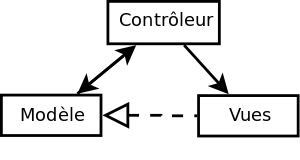
\includegraphics[scale=0.5]{images/MVC}
	\caption{\label{MVC} Patron de conception MVC}
	\end{center}
\end{figure}

\begin{figure}[!h]
	\begin{center}
	%% version 1.00, date 22/02/16, auteur Matthieu Martins-Baltar
% =================================================
% Set up a few colours
\colorlet{lcfree}{Gray}
\colorlet{lcnorm}{Gray}
\colorlet{lccong}{Gray}
\colorlet{lcinput}{Green}
\colorlet{lcoutput}{Red}
\colorlet{lcprero}{Blue}
\colorlet{lcpostro}{Purple}
\colorlet{lcforward}{Orange}
% -------------------------------------------------
% Set up a new layer for the debugging marks, and make sure it is on
% top
\pgfdeclarelayer{marx}
\pgfsetlayers{background,main,marx}
% A macro for marking coordinates (specific to the coordinate naming
% scheme used here). Swap the following 2 definitions to deactivate
% marks.
%\providecommand{\cmark}[2][]{%
%   \begin{pgfonlayer}{marx}
%   \node [nmark] at (c#2#1) {#2};
%  \end{pgfonlayer}{marx}
%  } 
\providecommand{\cmark}[2][]{\relax} 
% -------------------------------------------------

\begin{tikzpicture}[%
	auto,
    >=triangle 60,              % Nice arrows; your taste may be different
    start chain=going below,    % General flow is top-to-bottom
    node distance=6mm and 60mm, % Global setup of box spacing
    every join/.style={prero},   % Default linetype for connecting boxes
    ]
% ------------------------------------------------- 
% A few box styles 
% <on chain> *and* <on grid> reduce the need for manual relative
% positioning of nodes
\tikzset{
  base/.style={draw, on chain, on grid, align=center, minimum height=4ex},
  rule/.style={base, rectangle, text width=8em, font={\scriptsize}},
  proc/.style={base, rectangle, text width=8em},
  test/.style={base, diamond, aspect=2, text width=5em},
  term/.style={proc, rounded corners},
  % coord node style is used for placing corners of connecting lines
  coord/.style={coordinate, on chain, on grid, node distance=6mm and 25mm},
  % nmark node style is used for coordinate debugging marks
  %nmark/.style={draw, cyan, circle, font={\sffamily\bfseries}},
  % -------------------------------------------------
  % Connector line styles for different parts of the diagram
  prero/.style={->, draw, lcprero},
  input/.style={->, draw, lcinput},
  forward/.style={->, draw, lcforward},
  output/.style={->, draw, lcoutput},
  postro/.style={->, draw, lcpostro},
  norm/.style={->, draw, lcnorm},
  free/.style={->, draw, lcfree},
  cong/.style={->, draw, lccong},
  it/.style={font={\small\itshape}}
}
% -------------------------------------------------
% Start by placing the nodes
\node [term, fill=lcprero!25] (M)			{Modèle};
% Use join to connect a node to the previous one 
\node [term, fill=lcforward!25, join] (C)	{Logique métier\\ (Controleur)};
\node [term, fill=lcinput!25, join]	(V)		{Interface\\ (Vue)};

\node [term, fill=lcinput!25] (BD)			{Base de données};

\begin{pgfonlayer}{background}
	\node [term, join]	[fit = (M)(V)(C)]	{};
\end{pgfonlayer}

\node [term, fill=lcprero!25] (Nav)			{Navigateur};

%\node[obj,label={[name=id1-l]below:Outside}] (id1) at (2,2)  {}; 
%\begin{pgfonlayer}{background} 
%  \node[surround] (background) [fit = (id1)(id1-l)] {};
%\end{pgfonlayer}  

% No join for exits from test nodes - connections have more complex
% requirements
% We continue until all the blocks are positioned


% We position the next block explicitly as the first block in the
% second column.  The chain 'comes along with us'. The distance
% between columns has already been defined, so we don't need to
% specify it.




% -------------------------------------------------
% Now we place the coordinate nodes for the connectors with angles, or
% with annotations. We also mark them for debugging.


% -------------------------------------------------
% A couple of boxes have annotations
%\node [above=0mm of p4, it] {(Queue was empty)};
%\node [above=0mm of p8, it] {(Queue was not empty)};
% -------------------------------------------------
% All the other connections come out of tests and need annotating
% First, the straight north-south connections. In each case, we first
% draw a path with a (consistently positioned) annotation node, then
% we draw the arrow itself.


% ------------------------------------------------- 
% Now the straight east-west connections. To provide consistent
% positioning of the test exit annotations, we have positioned
% coordinates for the vertical part of the connectors. The annotation
% text is positioned on a path to the coordinate, and then the whole
% connector is drawn to its destination box.


% -------------------------------------------------
% Finally, the twisty connectors. Again, we place the annotation
% first, then draw the connector


% -------------------------------------------------
% A last flourish which breaks all the rules

% -------------------------------------------------
\end{tikzpicture}
% ================================================= % Marche pas :C
	\includegraphics[scale=0.6]{images/schemaArchitecture}
	\caption{\label{archi_schema} Schéma de l'architecture}
	\end{center}
\end{figure}